%---------------Grundeinstellungen---------------------------------------------------------
\documentclass[a4paper,12pt, DIV12]{scrartcl}
% Trennungen, Schriftsatz; neue Deutsche Rechtschreibung
\usepackage[ngerman]{babel}
\usepackage[T1]{fontenc} % Umlaute, Sonderzeichen...
% Für Betriebssysteme mit utf8-Codierung
\usepackage{ucs}
\usepackage[utf8x]{inputenc}
% ansonsten(z.B. Windows):
% \usepackage[ansinew]{inputenc}
%-----------------------------------------------------------------------------------------

%------------------Packete----------------------------------------------------------------
% Paket um Grafiken einzubinden. Evtl. muss unter Windows
% mit \usepackage[dvips]{graphicx} der dvips-Treiber für EPS-Grafiken geladen werden
\usepackage{graphicx}
\usepackage{subfigure}  % Bilder platzieren(z.B. nebeneinander)
\usepackage{multicol} % Paket für mehrspaltige Dokumente
\usepackage{float}    % Paket um Bilder in Fliess-Umgebungen einzubinden
\usepackage{amsmath}  % stellt die align-Umgebung zum Einrücken von Formeln zu Verfügung
\usepackage{amssymb}  % Extra mathematische Symbole
\usepackage{color}    % Farbdefinitionen
\usepackage{hyperref} % fuer klickbare Links
\usepackage{listings} % Quellcode farbig darstellen
\usepackage{lastpage} % Spezielles Paket um die Seiten zu zählen
\usepackage{scrpage2} % Kopf- und Fusszeilen
%\usepackage{pst-circ} % Elektronische Schaltungen
%\usepackage{pgfplots} % Für Diagramme
%----------------------------------------------------------------------------------------

%----------------Konfiguration-----------------------------------------------------------
\ihead{Inoffizielles Script zur Vorlesung Algebra 1, Prof. Schmidt}
%\chead{}
\ohead{Seite \thepage}
%\ifoot{}
\ofoot{Stand: \today}
%\cfoot{}
%\pagemark = Seitenzahl
\setheadsepline{1pt}    % Dicke der Trennlinie Kopfzeile - Text
\setfootsepline{0.5pt}  % Dicke der Trennlinie Fusszeile - Text
\pagestyle{scrheadings} % gemachte Einstellungen anwenden
\usepackage{setspace}   % Linienabstand
\onehalfspacing         % 1.5 Zeilenabstand; 1 = \singlespacing; 2 =
% \doublespacing
% schönere Hyperlinkfarben
\definecolor{darkred}{rgb}{0.5,0,0}
\definecolor{darkgreen}{rgb}{0,0.5,0}
\definecolor{darkblue}{rgb}{0,0,0.5}
\hypersetup{
  colorlinks,
  linkcolor=darkblue,
  filecolor=darkgreen,
  urlcolor=darkred,
  citecolor=darkblue
}
% Absatzeinzug
%\setlength{\parindent}{1em} % 1em = Grösse, die ein grosses M der aktuellen Schrift
\setlength{\parindent}{0pt}  % Kein Einzug, damit spart man sich die
% ganzen \\ nach einem Absatz!
%----------------------------------------------------------------------------------------

%----------------Beginn des eigentlichen Dokuments(also des Inhalts)---------------------
\begin{document}
\section{Mengen}
\subsection{Grundlegendes}
\subsubsection*{Was ist eine Menge?}
Eine Menge ist eine Zusammenfassung unterscheidbarer Objekte zu einer
Gesamtheit. Die Reihenfolge der Elemente ist unrelevant. Jedes Element ist einzigartig.

Seien A und B Elemente, dann gilt:
\begin{align}
  A = B    &\Leftrightarrow \{A, B\} = \{A\} \\
  A \neq B &\Leftrightarrow \{A, B\} \neq \{A\}
\end{align}
D.h. gleiche Elemente werden in Mengen nur einmal gezählt.
2 Mengen sind genau dann gleich, wenn sie die selben Elemente
enthalten.
\subsubsection*{Besondere Mengen}
Die Menge, die keine Elemente enthält, wird als die \emph{leere Menge} bezeichnet, das Symbol hierfür ist: $\{\}$ oder ${}\emptyset$.

Die \emph{Potenzmenge} ist die Vereinigung aller Teilmengen einer Menge.
Sie wird mit \(P(A)\) oder \(2^A\) bezeichnet. Jede Potenzmenge
enthält die leere Menge als Element.
\paragraph{Def.:} $P(A):= \{ U| {U}\subseteq{A} \}$
\paragraph{Beispiel:}
\begin{math}
{A = \{1,2,3\} }
\Rightarrow{2^A = \{ \emptyset, \{1\},\{2\},\{3\},\{1,2\},\{1,3\},A \} }
\end{math}
\newpage
\subsection{Mächtigkeit von Mengen}
Für endliche (abzählbare) Mengen ist die Mächtigkeit gleichzusetzen mit der Anzahl
der Elemente einer Menge. Für unendliche (nicht abzählbare) Mengen müssen andere
Definitionen getroffen werden, um deren Mächtigkeit zu beschreiben.
\paragraph{Man schreibt:}
\({}|{}A{}|{}\) oder \(\#A\)
\paragraph{Es gilt:}
\begin{math}
{}|{}2^A{}|{} = 2^{{}|{}A{}|{}}
\end{math}
\subsubsection*{Gleichmächtigkeit}
Seien A und B zwei beliebige Mengen.
Dann heißt A gleichmächtig zur Menge B, wenn eine Bijektion (\({f:A}\rightarrow{B}\)) gebildet
werden kann. Das bedeutet, dass eine Vorschrift existiert, welches
jedem Element der Menge A genau ein Element der Menge B zuordnet.
Dabei werden alle Elemente der Menge B einmal erfasst. Diese
Vorschrift ist umkehrbar.
\paragraph{Man schreibt:} \(\#A = \#B\) bzw. \(|A| = |B|\)
\paragraph*{Beispiele:}
\begin{math}
\#{\mathbb N} = \#{\mathbb Z} = \#{\mathbb Q}
\end{math}
\subparagraph{Erläuterung zu \(\#{\mathbb N} = \#{\mathbb Z}\):}
Der Einwand, dass die natürlichen Zahlen doch 'offensichtlich' (von der 0 abgesehen) doppelt so viele seien müssten, wie die ganzen Zahlen zählt bei diesen unendlichen Mengen nicht!
Stattdessen sollte man an die Definition der Gleichmächtigkeit denken: 2 Mengen sind dann gleich, wenn man eine eineindeutige(bijektive) Abbildung finden kann.

Hier ein Beispiel für eine solche Abbildung:
\begin{align*}
0 \rightarrow 0  \\
1 \rightarrow 1  \\
3 \rightarrow 2  \\
5 \rightarrow 3  \\
2 \rightarrow -1 \\
4 \rightarrow -2 \\
6 \rightarrow -3 \\
\end{align*}
Es werden also die 0 auf die 0, die ungeraden Zahlen auf die positiven Zahlen und die geraden Zahlen auf die negativen Zahlen abgebildet. Dies ist aufgrund der Unendlichkeit der beiden Mengen ohne Probleme möglich.

Auch für die rationalen Zahlen lässt sich ein solches Schema für eine Bijektion finden.
Hierauf geht ein Wikipedia-Artikel näher ein:

% J.S.: Wir sollten die Wikipedia-Artikel später in das Skript einarbeiten..
\url{http://de.wikipedia.org/wiki/Cantors_erstes_Diagonalargument}

Und auch bei der Frage, warum die reellen Zahlen nicht abzählbar sind, hilft Wikipedia:

\url{http://de.wikipedia.org/wiki/Cantors_zweites_Diagonalargument}

\subsection{Abbildungen}
%\subsubsection*{Einführendes Beispiel: Modellierung eines Netzwerks}
%Unterschiedliche Netzwerke wie soziale Netzwerke, Energienetzwerke oder U-Bahn-Linien-Netzwerke können mathematisch Modelliert werden.
%Hierzu ist ein Abstraktionsvorgang notwendig: Was haben diese Netzwerke gemeinsam?
%Mögliche Antwort: Elemente(Knoten) und Verbindungen
%Je nach konkretem Netzwerk sind müssen manche Dinge modelliert werden, andere nicht.
% Bsp.: U-Bahn Netz - nur Abfolge der Stationen und Dauer entscheident.
\subsubsection{Definition}
Seien A und B zwei Mengen.
Dann ist eine \emph{Abbildung} ein eindeutige Vorschrift, die jedem Element aus A genau ein Element aus B zuordnet.
Ein andere Bezeichnung für Abbildung ist \emph{Funktion}.
\subsubsection{Beispiel}
Sei $f:{A}\longrightarrow{B}$ eine Abbildungsvorschrift.
Dann ist:
\begin{align*}
   ker(f) := \{(a,c) \in A \times A\ | f(a)=f(c)\}
\end{align*}
eine Menge, der sogenannte Kern von f.

D.h. die Abbildung erzeugt sämtliche Paare von Elementen aus A, die den selben Funktionswert besitzen.
\footnote{Ich hoffe das stimmt auch, korrigiert mich hier bitte wenn
  ich das falsch verstanden habe!}
\newpage
\subsubsection{Typen von Abbildungen}
Seinen A und B zwei Mengen und $f:{A}\longrightarrow{B}$ eine Abbildungsvorschrift.
Dann gibt es 3 besondere Typen von Abbildungen:

\begin{description}
\item[surjektive Abbildung] \emph{alle} Elemente von B mindestens einmal erfassen
\item[injektive Abbildungen] alle Elemente von A erhalten \emph{unterschiedliche} Elemente aus B
\item[bijektive Abbildungen] \emph{surjektiv und injektiv} zu gleich: alle A erhalten genau ein B und alle B werden getroffen.
Dies impliziert die Umkehrbarkeit der Funktion. Eine Sonderform der bijektiven Abbildung ist die \emph{Identität}. Dabei wird jedes Element sich selbst zugeordnet.
\end{description}

\begin{figure}
\subfigure[surjektive Abbildung]{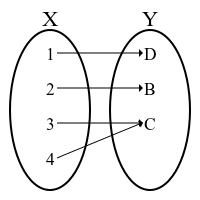
\includegraphics[width=4cm]{images/Surjection.png}}\hfill
\subfigure[injektive Abbildung]{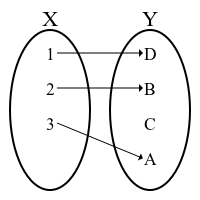
\includegraphics[width=4cm]{images/Injection.png}}\hfill
\subfigure[bijektive Abbildungen]{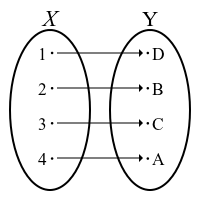
\includegraphics[width=4cm]{images/Bijection.png}}
\end{figure}

\subsubsection{Mächtigkeit einer Abbildung}
Seien A und B Mengen.
Dann bezeichne $B^A$ oder $Map(A,B)$ die Menge aller Abbildungen von A nach B.
\subparagraph*{Satz:}
Für A, B endliche Mengen gilt:
$$ |B^A| = {|B|}^{|A|} $$
\end{document}